\documentclass[a4paper]{article}

%%%%%%%%%%%%%%%%%%%%%%%%%%%%%%%%%%%%%%%%%%%%%%
\usepackage[T1]{fontenc}
\usepackage{geometry}
\geometry{a4paper,left=1.5cm,right=1cm,top=1cm,bottom=1cm}

\usepackage{graphicx}
\usepackage[absolute,overlay]{textpos}
\usepackage{eso-pic}               % image de fond
\usepackage{fontawesome5}
\usepackage[hidelinks]{hyperref}
\usepackage{tikz}
\usepackage{xcolor}
\usepackage{enumitem}
\setlist{nosep,leftmargin=6mm}
\usepackage{times}                % même police que votre exemple
\usepackage{array} 
\usepackage{tabularx}
\usepackage{ragged2e}
\let\origcolorbox\colorbox    % sauvegarde
\renewcommand{\colorbox}[2]{#2}% neutralise le fond
%%%%%%%%%%%%%%%%%%%%%%%%%%%%%%%%%%%%%%%%%%%%%%
%\definecolor{texcolor}{HTML}{e2e8f0}
\providecolor{sidetext}{rgb}{1,1,1}
\definecolor{maincolor}{HTML}{ffffff}

%%%%%%%%%%%%%%%%%%%%%%%%%%%%%%%%%%%%%%%%%
% — Ne changez pas le nom : « background.jpg » doit être présent
\AddToShipoutPictureBG*{%
  
\includegraphics[width=\paperwidth,height=\paperheight]{background.jpg}%
}

%%%%%%%%%%%%%%%%%%%%%%%%%%%%%%%%%%%%%%%%%
\newcommand{\fullrule}{\hspace{-1.5cm}\rule{\paperwidth}{0.4pt}}
\newcommand{\cvsection}[1]{%
  \vspace{6pt}\textbf{\Large #1}\par\vspace{2pt}}
\newcommand{\cicon}[1]{%
  \tikz[baseline]{\draw[fill=white] (0,0.1) circle[radius=0.1cm];}~#1}

\setlength{\parindent}{0pt}
%\color{texcolor}
%%%%%%%%%%%%%%%%%%%%%%%%%%%%%%%%%%%%%%%%%%%%%%%%%%%%%%%%%%%%%%
\begin{document}
\color{white}
% ---------- Photo ------------------------------------------------
\begin{textblock*}{4cm}(0.2cm,0.3cm)
  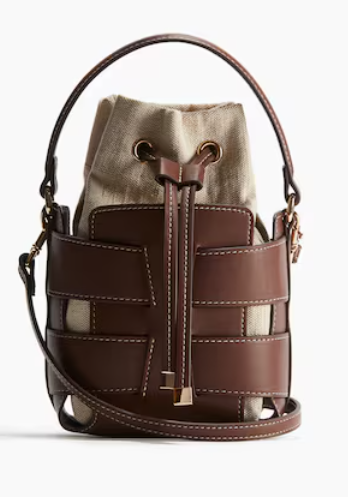
\includegraphics[width=2.5cm,clip,keepaspectratio]{e8457e633ca141a198e9f797fab7ef3b.png}
\end{textblock*}

% ---------- En-tête ---------------------------------------------
\begin{center}
  {\fontsize{44pt}{24pt}\selectfont\bfseries Judikael Mourouvin}

  \bigskip
  {\Large Alternant Marketing Digital \& Support Informatique}

  \bigskip\bigskip
  \faMapMarker~Route de Cocoyer\ 97190 Gosier
  \quad\faEnvelope~\href{mailto:jkmou971@gmail.com}{jkmou971@gmail.com}

  \bigskip
  % Badge LinkedIn (retirez-le si inutile)
  \faPhone~ +590 0690 91 14 48
  \quad \faLinkedin\ \href{}{}
 

  \vspace{-0.3cm}
  \fullrule
\end{center}

% ---------- Profil ----------------------------------------------
\cvsection{Profil}
Passionné par l’informatique et le marketing digital, j’ai développé une expertise en configuration de postes, maintenance et support aux utilisateurs. Mon année d’alternance à la DSI de la Mairie du Gosier m’a permis de piloter des projets numériques et de former les agents aux nouveaux outils. Orienté résultats et service client, je cherche désormais à mettre mes compétences techniques et marketing au service de nouveaux défis avec rigueur et efficacité.

\medskip\fullrule

% ---------- Expérience ------------------------------------------
\cvsection{Expérience}
\hspace*{1.3cm}%

\colorbox{maincolor}{%
  \begin{minipage}{\linewidth}
    \textbf{Alternant en Marketing Digital} \\ Mairie du Gosier – DSI \\ 2023-2024
    \begin{itemize}
      \item Géré des projets numériques améliorant l’efficacité des services municipaux \item Analysé les besoins et déployé des solutions adaptées aux utilisateurs \item Assuré support et formation favorisant l’adoption des outils digitaux
    \end{itemize}
  \end{minipage}}

\vspace{3mm}


\colorbox{maincolor}{%
  \begin{minipage}{\linewidth}
    \textbf{Animateur de la zone informatique} \\ Pôle Emploi, Gosier \\ 2022-2023
    \begin{itemize}
      \item Fournit un support technique quotidien garantissant la continuité de service \item Configuré et maintenu les postes, réduisant les pannes matérielles \item Diagnostiqué et résolu les incidents pour rétablir rapidement la productivité
    \end{itemize}
  \end{minipage}}

\vspace{3mm}


\colorbox{maincolor}{%
  \begin{minipage}{\linewidth}
    \textbf{Stagiaire Informaticien} \\ NUMERIKA, Baie-Mahault \\ 2020-2021
    \begin{itemize}
      \item Installé et entretenu les équipements informatiques des clients \item Assuré le support utilisateurs pour maintenir la disponibilité des systèmes
    \end{itemize}
  \end{minipage}}

\medskip\fullrule

% ---------- Éducation -------------------------------------------
\cvsection{Éducation}
\hspace*{1.3cm}%

    \begin{tabularx}{\linewidth}{@{}c >{\RaggedRight\arraybackslash}X@{}}
    \textcolor{sidetext}{\faGraduationCap} &
    \textbf{Bachelor Marketing Digital} \\
    & CFA IUTS \\
    & \textit{2023-2024} \\
    \end{tabularx}
    \begin{itemize}[leftmargin=*]
  \item Stratégies de marketing en ligne (SEO, SEA, réseaux sociaux)
  \item Analyse de données et optimisation des campagnes digitales
  \item Gestion de projets digitaux et veille technologique
\end{itemize}
\vspace{3mm}

    \begin{tabularx}{\linewidth}{@{}c >{\RaggedRight\arraybackslash}X@{}}
    \textcolor{sidetext}{\faGraduationCap} &
    \textbf{BTS Système Numérique option Informatique et Réseaux} \\
    & Lycée de Chevalier Saint Georges, Abymes \\
    & \textit{2019-2021} \\
    \end{tabularx}
    \begin{itemize}[leftmargin=*]
  \item Administration de systèmes et réseaux
  \item Programmation et intégration de solutions numériques
  \item Support et maintenance matériels et logiciels
\end{itemize}

\medskip\fullrule

% ---------- Compétences -----------------------------------------
\cvsection{Compétences}
\hspace*{2.2cm}%
\begin{tabular}{@{}p{0.25\linewidth}p{0.18\linewidth}p{0.18\linewidth}p{0.18\linewidth}}\cicon Administration & \cicon Réseaux & \cicon Support & \cicon Maintenance \\
\cicon Diagnostic & \cicon Marketing & \cicon Digital & \cicon Configuration \\
\cicon Assistance & \cicon Formation & ~ & ~ \\\end{tabular}   % grille 3 lignes × 4 colonnes

\end{document}
